\documentclass[11pt]{article}
\usepackage{fullpage}
\usepackage{url}
\usepackage{color}
\usepackage{amsmath, amssymb}
\usepackage{hyperref}
\usepackage{geometry}
\usepackage{adjustbox}
\usepackage{multirow}
\usepackage{setspace}
\usepackage{listings}
\usepackage{hyperref}
\newgeometry{vmargin={15mm}, hmargin={12mm,17mm}}
\textheight=8.85in

\hypersetup{
	colorlinks=true,
	linkcolor=blue,
	filecolor=magenta,      
	urlcolor=blue,
}

\renewcommand{\arraystretch}{1.5}
\setlength{\tabcolsep}{12pt}
\usepackage{float}

\doublespacing

\pagestyle{myheadings}

\definecolor{codebg}{gray}{0.95}

\lstset{ 
	language=Matlab,                		% choose the language of the code
	%	basicstyle=10pt,       				% the size of the fonts that are used for the code
	numbers=left,                  			% where to put the line-numbers
	numberstyle=\footnotesize,      		% the size of the fonts that are used for the line-numbers
	stepnumber=1,                   			% the step between two line-numbers. If it's 1 each line will be numbered
	numbersep=5pt,                  		% how far the line-numbers are from the code
	backgroundcolor=\color{codebg},  	% choose the background color. You must add \usepackage{color}
	showspaces=false,               		% show spaces adding particular underscores
	showstringspaces=false,         		% underline spaces within strings
	showtabs=false,                 			% show tabs within strings adding particular underscores
	%	frame=single,	                			% adds a frame around the code
	%	tabsize=2,                				% sets default tabsize to 2 spaces
	%	captionpos=b,                   			% sets the caption-position to bottom
	breaklines=true,                			% sets automatic line breaking
	breakatwhitespace=false,        		% sets if automatic breaks should only happen at whitespace
	escapeinside={\%*}{*)}          		% if you want to add a comment within your code
}



	\title{\textbf{CSE 847 Home Assignment 3}}
	\author{\textbf{\textit{Submitted by:}} Ritam Guha (MSU ID: guharita)}
	\date{\textbf{\textit{Date:}} March 19, 2021}


\begin{document}

\maketitle

\thispagestyle {empty}

\newcommand{\lsp}[1]{\large\renewcommand{\baselinestretch}{#1}\normalsize}
\newcommand{\hsp}{\hspace{.2in}}
\newcommand{\comment}[1]{}
\newtheorem{thm}{Theorem}[section]
\newtheorem{lem}{Lemma}[section]
\newtheorem{cor}{Corollary}[section]
\newtheorem{prop}{Proposition}[section]
\newtheorem{problem}{Problem}[section]

\newcommand{\R}{{\rm\hbox{I\kern-.15em R}}}
\newcommand{\IR}{{\rm\hbox{I\kern-.15em R}}}
\newcommand{\II}{{\rm\hbox{I\kern-.15em I}}}
\newcommand{\IN}{{\rm\hbox{I\kern-.15em N}}}
\newcommand{\IZ}{{\sf\hbox{Z\kern-.40em Z}}}
\newcommand{\IS}{{\rm\hbox{S\kern-.45em S}}}
\newcommand{\Real}{I\!\!R}


\newcommand{\linesep}{\vspace{.2cm}\hrule\vspace{0.2cm}}
\newcommand{\categorysep}{\vspace{0.5cm}}
\newcommand{\entrysep}{\vspace{0cm}}

\newcommand{\category}[1]{\categorysep
                  \noindent {\bf \large #1}
              \linesep}

\pagestyle{empty}

\section{Linear Algebra III}

\begin{enumerate}

\item (10 points) Let $A \in \IR^{m \times n}$ be a matrix of rank $n$. Prove that $\| A(A^T A)^{-1} A^T \|_2 = 1$.\\
\textbf{Response:}\\
$A$ is a full rank matrix. So, SVD of A looks like:\\
$A = \begin{pmatrix} U_1 & U_2 \end{pmatrix} \begin{pmatrix}\Sigma \\ 0 \end{pmatrix} \begin{pmatrix} V^T \end{pmatrix}$\\
where $U_1 \in \IR^{m \times n}$, $U_2 \in \IR^{m \times (m-n)}$ have orthogonal columns , $\Sigma \in \IR^{n \times n}$ is a  diagonal matrix and $V \in \IR^{n \times n}$ is orthogonal. Simplifying $A$ gives us:\\
$A = U_1 \Sigma V^T$\\
 Plugging in this form in the given expression, we get:\\
 $||U_1 \Sigma V^T ((U_1 \Sigma V^T)^T U_1 \Sigma V^T)^{-1} (U_1 \Sigma V^T)^T||_2$\\
 $= ||U_1 \Sigma V^T (V \Sigma U_1^T U_1 \Sigma V^T)^{-1} V \Sigma U_1^T||_2$\\
 $= ||U_1 \Sigma V^T (V \Sigma^2 V^T)^{-1} V \Sigma U_1^T||_2$\\
 $= ||U_1 \Sigma V^T (V^T)^{-1} \Sigma^{-2} V^{-1} V \Sigma U_1^T||_2$\\
 $= ||U_1 \Sigma  \Sigma^{-2} \Sigma U_1^T||_2$\\
 $= ||U_1 U_1^T||_2$\\
 $= ||\II||_2$\\

 According to the definition of 2-norm of matrices, $||A||_2$ is the square root of the largest eigen value of $A^T A$.\\
 Square root of the Largest eigen value of $\II \II$ is 1. [Proved]

\item (10 points) Let $A$ and $B$ be two positive semi-definite matrices in $\IR^{n \times n}$. Prove or disprove: 
$A$ and $B$ are PSDs. So, for any $v \epsilon \IR^n$, $v^T A v$ and $v^T B v$ should be greater than or equal to $0$.
\begin{enumerate}
\item $A+B$ is positive semi-definite\\
\textbf{Response:}\\
$v^T (A+B) v$\\
$= v^T A v + v^T B v$\\
where $v^T A v \geq 0$ and $v^T B v \geq 0$\\
So, $v^T (A+B) v \geq 0$\\
Hence, it is a PSD.  \\

\item $AB$ is positive semi-definite\\
\textbf{Response:}\\
$AB$ is not always postive semi-definite. While doing multiplication of matrices, the symmetry does not hold always. But according to the definition of PSD matrices, it should be symmetric. For an example, consider the following PSD matrices as $A$ and $B$.\\
$A = \begin{pmatrix}1 & 4\\ 4 & 16\\\end{pmatrix}$,
$B  = \begin{pmatrix}4 & -6\\ -6 & 9\\\end{pmatrix}$\\
$AB = \begin{pmatrix}-20 & 30\\ -80 & 120\\\end{pmatrix}$\\
So, $AB$ is not symmetric. Now let's consider $v$ as $\begin{pmatrix}1\\ 0\\\end{pmatrix}$\\
$\begin{pmatrix}1 & 0\\\end{pmatrix} \begin{pmatrix}-20 & 30\\ -80 & 120\\\end{pmatrix}        \begin{pmatrix}1\\ 0\\\end{pmatrix} = -20$\\
So, $AB$ is not a PSD matrix. 
Using this counter example, it is proved that $AB$ may not be a PSD.\\

\item $B^T$ is positive semi-definite\\
\textbf{Response:}\\
By definition of positive semi-definite matrices, they should be symmetric.\\
$B$ is a PSD matrix, so it should be symmetric.\\
$B = B^T$\\
So, $B^T$ is also a PSD matrix.\\
\end{enumerate} 

\end{enumerate}


\section{Linear Classification} 

Questions in the textbook Pattern Recognition and Machine Learning:
\begin{enumerate}
\item (10 points) Page 220, Question 4.1\\
\textbf{Response:}\\
The convex hull for a set of data points ${x_n}$ is given by:\\
$\textbf{x} = \displaystyle \sum_n \alpha_n x_n$ where $\displaystyle \sum_n \alpha_n = 1$\\
If there are two intersecting convex hulls $\textbf{x}$, $\textbf{y}$, for some combinations of $\alpha_n \geq 0$ and $\beta_n \geq 0$, the following equality should hold:\\
$\displaystyle \sum_n \alpha_n x_n = \displaystyle \sum_n \beta_n y_n = c$ [A common point on the convex hull]\\

Let's consider that these two intersecting convex hulls are linearly separable. Then from the definition of linear separability, we can say:\\
$\hat{w}^T x_n + w_0 > 0$\\
$\hat{w}^T y_n + w_0 < 0$\\

$\hat{w}^T c + w_0$\\
$= \displaystyle \hat{w}^T (\sum_n \alpha_n x_n) + (\sum_n \alpha_n) w_0$  [As $\displaystyle \sum_n \alpha_n = 1$]\\
$= \displaystyle(\sum_n \alpha_n \hat{w}^T x_n) + \sum_n \alpha_n w_0$\\
$= \displaystyle \sum_n \alpha_n (\hat{w}^T x_n + w_0)$\\ 
As $\hat{w}^T x_n + w_0 > 0$, $\hat{w}^T c + w_0 > 0$ 

If we use $c = \sum_n \beta_n y_n$, $\hat{w}^T c + w_0 = \displaystyle \sum_n \beta_n (\hat{w}^T y_n + w_0)$.\\
Then this becomes $<0$ because $\hat{w}^T y_n + w_0 < 0$.\\
This leads to a contradiction. So, our assumption that the intersecting convex hulls are linearly separable was wrong.\\
\textbf{If convex hulls of two sets of points intersect, they are not linearly separable.}\\

In the same way, we can show that \textbf{If two sets of points are linearly separable, their convex hulls cannot intersect.}\\

\item (10 points) Page 221, Question 4.5\\
\textbf{Response:}\\
The given expressions are:\\
$y = \bold{w^T x}$\\
$m_k = \bold{w^T m_k}$\\
$\displaystyle s_k^2 = \sum_{n \epsilon C_k} (y_n - m_k)^2$\\

The fisher criterion can be represented as:\\
$\displaystyle J(w) = \frac{(m_2  - m_1)^2}{s_1^2 + s_2^2}$\\

From the given expressions, we can derive the follwoing expressions:\\
$m_1 = \bold{w^Tm_1}$\\
$m_2 = \bold{w^Tm_2}$\\

\begin{flalign*}
(m_2 - m_1)^2  &= (\bold{w^T (m_2 - m_1)})^2 &\\
               &= \bold{w^T (m_2 - m_1) (w^T (m_2 - m_1))^T}\\
               &= \bold{w^T (m_2 - m_1) (m_2 - m_1)^T w}\\
               &= \bold{w^T S_B w}\\
\end{flalign*}
where $S_B = (m_2 - m_1) (m_2 - m_1)^T$\\

\begin{flalign*}
\displaystyle s_1^2 &= \sum_{n \epsilon C_1} (y_n - m_1)^2 &\\
                    &= \sum_{n \epsilon C_1} (\bold{w^T x_n - w^T m_1})^2 \\
                    &= \sum_{n \epsilon C_1} (\bold{w^T(x_n - m_1)})^2\\
                    &= \sum_{n \epsilon C_1} (\bold{w^T(x_n - m_1) (w^T(x_n - m_1))^T})\\
                    &= \sum_{n \epsilon C_1} (\bold{w^T (x_n - m_1)(x_n - m_1)^T w})\\
                    &= \bold{w^T} (\sum_{n \epsilon C_1} \bold{(x_n - m_1)(x_n - m_1)^T}) \bold{w}\\
\end{flalign*}

Similarly $s_2^2 = \bold{w^T} (\sum_{n \epsilon C_2} \bold{(x_n - m_2)(x_n - m_2)^T}) \bold{w}$

So,\\
\begin{flalign*}
\displaystyle s_1^2 + s_2^2 &= \bold{w^T} (\sum_{n \epsilon C_1} \bold{(x_n - m_1)(x_n - m_1)^T}) \bold{w} + \bold{w^T} (\sum_{n \epsilon C_2} \bold{(x_n - m_2)(x_n - m_2)^T}) \bold{w} &\\
        &= \bold{w^T} (\sum_{n \epsilon C_1} \bold{(x_n - m_1)(x_n - m_1)^T} + \sum_{n \epsilon C_2} \bold{(x_n - m_2)(x_n - m_2)^T)} \bold{w}\\
        &= \bold{w^T S_w w}\\
\end{flalign*}
   
The fisher criterion then becomes:
\begin{flalign*}
    \displaystyle J(w) &= \frac{(m_2 - m_1)^2}{s_1^2 + s_2^2} &\\
                       &= \frac{\bold{w^T S_B w}}{\bold{w^T S_w w}}
\end{flalign*}
    
Thus, the two forms are equivalent. 
\item (10 points) Page 221, Question 4.6\\
\textbf{Response:}
Equation 4.3 is given by:\\
$\displaystyle \sum_{i=1}^N (w^T x_n + w_0 - t_n) x_n = 0$
We can simplify it using equations (4.34), (4.35), (4.36) in the following manner:\\
$\displaystyle \Rightarrow \sum_{i=1}^N w^T x_n x_n + \sum_{i=1}^N w_0 x_n - \sum_{i=1}^N t_n x_n = 0$\\
$\displaystyle \Rightarrow \sum_{i=1}^N w^T x_n x_n - w^T m \sum_{i=1}^N x_n - (\sum_{n \epsilon C_1} \frac{N}{N_1} x_n + \sum_{n \epsilon C_2} -\frac{N}{N_2} x_n) = 0$ [Using equation 4.34, we get $w_0 = -w^T m$ and using different representations of $t_n$ for the two classes]\\
$\displaystyle \Rightarrow \sum_{i=1}^N w^T x_n x_n - w^T m Nm - (\frac{N}{N_1} \sum_{n \epsilon C_1} x_n - \frac{N}{N_2} \sum_{n \epsilon C_2} x_n) = 0$ [where $m$ is the mean of the entire dataset]\\
$\displaystyle \Rightarrow \sum_{i=1}^N w^T x_n x_n - N w^T m m - (\frac{N}{N_1} N_1m_1 - \frac{N}{N_2} N_2 m_2) = 0$\\
$\displaystyle \Rightarrow \sum_{i=1}^N x_n x_n^T w - N m m^T w - N(m_1 - m_2) = 0$ [As $w^T x_n$ and $w^t m$ are scalars]\\
$\displaystyle \Rightarrow \sum_{i=1}^N x_n x_n^T w - N m m^T w = N(m_1 - m_2)$\\
$\displaystyle \Rightarrow (\sum_{i=1}^N x_n x_n^T  - N m m^T) w = N(m_1 - m_2)$\\
$\displaystyle \Rightarrow (\sum_{i=1}^N x_n x_n^T  - N (\frac{1}{N} (N_1 m_1 + N_2 m_2)) (\frac{1}{N}(N_1 m_1 + N_2 m_2)^T)) w = N(m_1 - m_2)$ [From equation (4.36), $\displaystyle m=\frac{1}{N} (N_1m_1 + N_2m_2)]$ \\ 
$\displaystyle \Rightarrow (\sum_{i=1}^N x_n x_n^T  - \frac{1}{N}(N_1 m_1 + N_2 m_2) (N_1 m_1^T + N_2 m_2^T)) w = N(m_1 - m_2)$\\
$\displaystyle \Rightarrow (\sum_{i=1}^N x_n x_n^T  - \frac{1}{N}(N_1^2||m_1||^2 + N_2^2||m_2||^2 + 2 N_1 N_2 m_1^T m_2)) w = N(m_1 - m_2)$\\
$\displaystyle \Rightarrow (\sum_{i=1}^N x_n x_n^T  - \frac{N_1^2}{N}||m_1||^2 - \frac{N_2^2}{N}||m_2||^2 - 2 \frac{N_1 N_2}{N} m_1^T m_2) w = N(m_1 - m_2)$\\
$\displaystyle \Rightarrow (\sum_{i=1}^N x_n x_n^T  - \frac{N_1^2}{N}||m_1||^2 - \frac{N_2^2}{N}||m_2||^2 - \frac{N_1 N_2}{N} ||m_1||^2 - \frac{N_1 N_2}{N} ||m_2||^2  + \frac{N_1 N_2}{N} ||m_1||^2 + \frac{N_1 N_2}{N} ||m_2||^2 - 2 \frac{N_1 N_2}{N} m_1^T m_2) w = N(m_1 - m_2)$\\
$\displaystyle \Rightarrow (\sum_{i=1}^N x_n x_n^T  - \frac{N_1^2}{N}||m_1||^2 - \frac{N_2^2}{N}||m_2||^2 - \frac{N_1 N_2}{N} ||m_1||^2 - \frac{N_1 N_2}{N} ||m_2||^2  + (\frac{N_1 N_2}{N} ||m_1||^2 + \frac{N_1 N_2}{N} ||m_2||^2 - 2 \frac{N_1 N_2}{N} m_1^T m_2)) w = N(m_1 - m_2)$\\
$\displaystyle \Rightarrow (\sum_{i=1}^N x_n x_n^T  - \frac{N_1^2}{N}||m_1||^2 - \frac{N_2^2}{N}||m_2||^2 - \frac{N_1 N_2}{N} ||m_1||^2 - \frac{N_1 N_2}{N} ||m_2||^2  + \frac{N_1 N_2}{N} (m_2 - m_1) (m_2 - m_1)^T) w = N(m_1 - m_2)$\\
$\displaystyle \Rightarrow (\sum_{i=1}^N x_n x_n^T  - \frac{N_1}{N}(N_1 + N_2)||m_1||^2 - \frac{N_2}{N} (N_2 + N_1)||m_2||^2+ \frac{N_1 N_2}{N} S_B) w = N(m_1 - m_2)$\\
$\displaystyle \Rightarrow (\sum_{i=1}^N x_n x_n^T  - N_1 ||m_1||^2 - N_2 ||m_2||^2+ \frac{N_1 N_2}{N} S_B) w = N(m_1 - m_2)$\\
$\displaystyle \Rightarrow (\sum_{n \epsilon C_1} (x_n x_n^T  + ||m_1||^2 - 2 m_1 x_n^T)  + \sum_{n \epsilon C_2} (x_n x_n^T  + ||m_2||^2 - 2 m_2 x_n^T) - 2N_1||m_1||^2 - 2N_2||m_2||^2 +  \sum_{n \epsilon C_1}2m_1 x_n^T +  \sum_{n \epsilon C_1}2m_2 x_n^T + \frac{N_1 N_2}{N} S_B) w = N(m_1 - m_2)$\\
$\displaystyle \Rightarrow (\sum_{n \epsilon C_1} (x_n - m_1)(x_n - m_1)^T  + \sum_{n \epsilon C_2} (x_n - m_2)(x_n - m_2)^T - 2N_1||m_1||^2 - 2N_2||m_2||^2 +  2N_1||m_1||^2 +  2N_2||m_2||^2 + \frac{N_1 N_2}{N} S_B) w = N(m_1 - m_2)$\\
$\displaystyle \Rightarrow (S_w + \frac{N_1 N_2}{N} S_B) w = N(m_1 - m_2)$ [Proved]\\
\item (10 points) Page 222, Question 4.15\\
\textbf{Response:}\\
The hessian matrix is given by:\\
$\displaystyle \textbf{H} = \sum_{n=1}^N y_n (1-y_n) \phi_n \phi_n^T$\\
If we want to show that $\textbf{H}$ is positive definite, for any non-zero vector $v$ in $\IR^M$, $v^T \textbf{H} v$ should be greater than $0$.\\
$v^T \textbf{H} v$\\
$= v^T (\sum_{n=1}^N y_n (1-y_n) \phi_n \phi_n^T)  v$\\
$= \sum_{n=1}^N y_n (1-y_n) (v^T \phi_n) (\phi_n^T v)$\\
$= \sum_{n=1}^N y_n (1-y_n) ||v^T \phi_n||_2^2$\\

In this expression, $y_n \epsilon (0,1)$, so $y_n (1 - y_n) > 0$. $v^T \phi_n$ can be treated as a linear combination of columns of $\Phi$. As $\Phi$ is the design matrix, we can assume it to have linearly independent columns. Linear combination of linearly independent columns is only zero when the scalars used for the linear combination (here $v$) are zeros. But, $v$ is a non-zero vector, so the linear combination of the columns of $\Phi$ cannot be negative which makes linear combination to be positive. So, there should be at least one $n$ for which $v^T \phi_n$ is greater than $0$ which makes $v^T \bold{H} v > 0$. So, by definition of PD matrices, $\textbf{H}$ is a PD matrix.\\ 

So, we can see that the second derivative of the error function with respect to $w$ is a PD matrix. This leads to the fact that the error function should be a convex (concave upwards) function of $w$.  Hence, according to the properties of convex functions, it has a unique minimum value.
\end{enumerate}

\section{Linear Regression: Experiment} 

 (40 points) In this part of homework you will explore the ridge regression and the effects of
$\ell_2$-norm regularization. You are to implement a MATLAB solver for ridge regression:
$$ \min_w \frac{1}{2}\|Xw - y\|_2^2 + \frac{\lambda}{2} \|w\|_2^2. $$
You are not allowed to use the integrated ridge regression in MATLAB.
You will use your solver to investigate the effects of the regularization on the \textsc{Diabetes}\footnote{\url{https://github.com/jiayuzhou/CSE847/blob/master/data/diabetes.mat?raw=true}}
dataset, and study the cross validation procedure.

\begin{enumerate}
\item Implement the ridge regression solver.  
\item Train regression models on the \textsc{Diabetes} dataset using 
the training data (x\_train, y\_train variables in the data file). 
Vary the $\lambda$ from ${1e-5}, {1e-4}, {1e-3}, {1e-2}, {1e-1}, 1, 10$ (In 
Matlab $1e-1$ means $0.1$). 
Compute training error (predict y\_train given X\_train), testing error (predict y\_test given X\_test) for each $\lambda$. 
The error is measured by mean squared error (MSE):
$$
\mbox{MSE} = \frac{1}{N}\sum_{i=1}^N (y_i - \hat y_i)^2,
$$
where $N$ is the number of samples on which the error is computed, $y_i$ 
is ground truth, and $\hat y_i$ is the prediction from data points 
given model $w$. 
\item Perform 5-fold cross validation on the training data to estimate the best $\lambda$ from training data.
\end{enumerate}

In the homework, attach a brief report. In the report you need to
discuss your findings in the experiment, include a plot showing how
training/testing error changes when you vary the parameter $\lambda$ (use log
scale on $\lambda$). In the same plot, show the best $\lambda$ obtained from
your 5-fold cross validation procedure. Submit the MATLAB code (do add some comments in your code for others to understand your code) to the D2L along with your report. 

\textbf{Response:}
For the regression problem, we can find the expression of the weights as:

\begin{equation}
	w = (\Phi^T \Phi + \lambda \II)^{-1} \Phi^T t
	\label{Eq:weights}
\end{equation}

where $\Phi$ is the design matrix and $t$ is the target vector. The weights are computed from the training matrix and then applied over test data to compute the predictions. Based on the predictions, every such model provides a MSE which can be used as the quality indicator of the model.\\

The model has one hyperparamter which is $\lambda$. In order to get one optimal value of $\lambda$, $k$-fold cross-validation is performed. After getting an optimal value of $\lambda$, that is used to build the model which is finally applied over the test data. The entire result of this experimentation is tabulated in Table 1.\\

Different types of normalization techniques are also used on the data to measure the change in errors based on different types of normalizations. For this purpose, $5$ types of normalization techniques are used apart from the non-normalized scenario. These normalization techniques are available in \textit{MATLAB} under the names: `range', `scale', `zscore', `norm', `center'. Each of these normalization techniques use different methods to scale the data. The description of each type of normalization can be found in the \href{https://in.mathworks.com/help/matlab/ref/double.normalize.html}{\textit{MathWorks} documentation}.\\ 

In Table 1, for each of the $\lambda$s, Train Error and Test Error refer to the MSE values over the training data and testing data for the model generated using Equation \ref{Eq:weights} using that $\lambda$. The Train Error is always less than the Test Error because Training data is used to build the model but the Test data is completely unseen to the model. So, Test data is used to evaluate the generalization of different models. Train Error and Test Error are computed before cross-validation with all the possible models.\\  

After performing cross-validation,  the best $\lambda$ value out of the mentioned possiblilities are calculated for every normalization procedure. We can see that the values change depending on the normalization technique used. So, normalization can affect the selection of the model which is really interesting. We can see that for every scenario, the regularized version is providing better Mean Square error compared to the non-regularised variant. To check the correctness of the code, I also used the \textit{MATLAB} integrated ridge regression for benchmarking and founf out it is performing in a similar manner with little variance. 

\begin{table}[H]
	\centering
	\label{Tab:Results}
	\begin{adjustbox}{width=0.75\paperwidth}
		\begin{tabular}{| c | c |cccccc|}
			\hline
			\centering
			& \multirow{2}{*}{\textbf{Error Type}} & \multicolumn{6}{|c|}{\textbf{Normalization Type}}\\ \cline{3-8}
			&  & \textbf{None} & \textbf{Range} & \textbf{Scale} & \textbf{Z-score} & \textbf{Norm} & \textbf{Center} \\ \hline
			\multirow{2}{*}{$\lambda$=1e-6} & Train Error & 19560.40391 & 0.021933 & 3.366411 & 0.385461 & 0.002891 & 2189.03486 \\ 
			& Test Error & 93835.00672 & 3.589247 & 1005.224421 & 4.338947 & 0.056803 & 3558.254969 \\ \hline
			\multirow{2}{*}{$\lambda$=1e-5} & Train Error & 19695.35482 & 0.021947 & 3.380637 & 0.385516 & 0.002906 & 2194.171893 \\ 
			& Test Error & 76911.07209 & 1.621412 & 462.882938 & 2.244155 & 0.032902 & 3514.411567 \\ \hline
			\multirow{2}{*}{$\lambda$=1e-4} & Train Error & 20060.11614 & 0.022058 & 3.431649 & 0.385708 & 0.002956 & 2209.43153 \\ 
			& Test Error & 57531.76027 & 0.123865 & 80.669288 & 0.808274 & 0.013571 & 3483.224263 \\ \hline
			\multirow{2}{*}{$\lambda$=1e-3} & Train Error & 20384.66425 & 0.022171 & 3.451689 & 0.385887 & 0.003003 & 2227.638985 \\ 
			& Test Error & 49060.59804 & 0.107295 & 40.584322 & 0.649208 & 0.0083 & 3285.303421 \\ \hline
			\multirow{2}{*}{$\lambda$=1e-2} & Train Error & 20918.86518 & 0.022419 & 3.493135 & 0.387634 & 0.003069 & 2306.837688 \\ 
			& Test Error & 44405.1394 & 0.055242 & 18.906226 & 0.644382 & 0.007227 & 2951.255302 \\ \hline
			\multirow{2}{*}{$\lambda$=1e-1} & Train Error & 22075.71567 & 0.023389 & 3.556196 & 0.390146 & 0.003194 & 2511.476379 \\ 
			& Test Error & 36994.69673 & 0.035062 & 9.140952 & 0.636367 & 0.006359 & 2852.421846 \\ \hline
			\multirow{2}{*}{$\lambda$=1} & Train Error & 24730.73933 & 0.025154 & 3.620571 & 0.39539 & 0.003527 & 3288.941082 \\ 
			& Test Error & 30517.77394 & 0.029653 & 7.306174 & 0.543775 & 0.005187 & 3510.851314 \\ \hline
			\multirow{2}{*}{$\lambda$=10} & Train Error & 27165.12613 & 0.03021 & 3.728976 & 0.415413 & 0.003947 & 4917.706446 \\ 
			& Test Error & 30057.3035 & 0.033097 & 6.58842 & 0.470815 & 0.004905 & 5390.676364 \\ \hline
			\multirow{2}{*}{$\lambda$=100} & Train Error & 27827.97731 & 0.045432 &	4.009522 &	0.465563 &	0.004107 &	5556.667563 \\ 
			& Test Error & 30414.29643 & 0.048561 &	5.430243 & 0.474178 & 0.004982 & 6136.625862 \\ \hline
			\multicolumn{2}{|c|}{Best $\lambda$ according to CV-MSE} & 10 & 1 & 100 & 100 & 100 & 0.1 \\ \hline
			\multicolumn{2}{|c|}{MSE for Non-Regularized version} & 106775.3616 & 3.972377 & 1132.597799 & 4.838317 & 1.160637 & 3630.528184 \\ \hline
			\multicolumn{2}{|c|}{MSE for Ridge Regularized version}  & 30057.3035 & 0.029653 & 6.081624 & 0.461673 & 0.004905 & 2852.421846 \\ \hline
			\multicolumn{2}{|c|}{MSE for MATLAB integrated Ridge Regularized version}  & 30145.62543 & 0.094501 & 4.25334 & 0.461673 & 0.004928 & 5911.960252 \\ \hline
		\end{tabular}
	\end{adjustbox}
	
	\caption{Results for the Linear Regression Experimentation.}
\end{table}

In Figure \ref{Fig: MSE_Plot}, the average MSE values during cross-valdiation are plotted for different values of $\lambda$ for various Normalization techniques. 

\begin{figure}[H]
	\centering
	\begin{adjustbox}{width=0.8\paperwidth}
		\begin{tabular}{c c}
			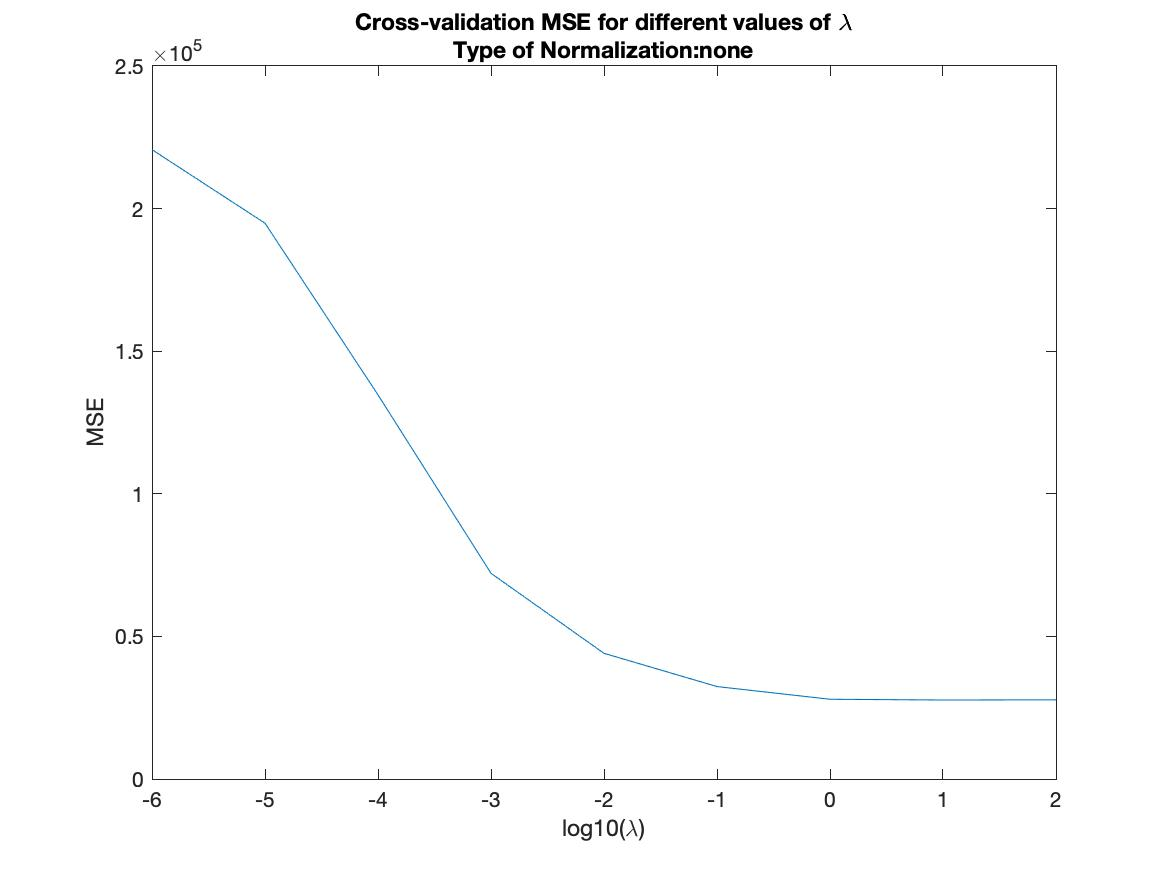
\includegraphics{Codes/MSE_Plots_none.jpg} & 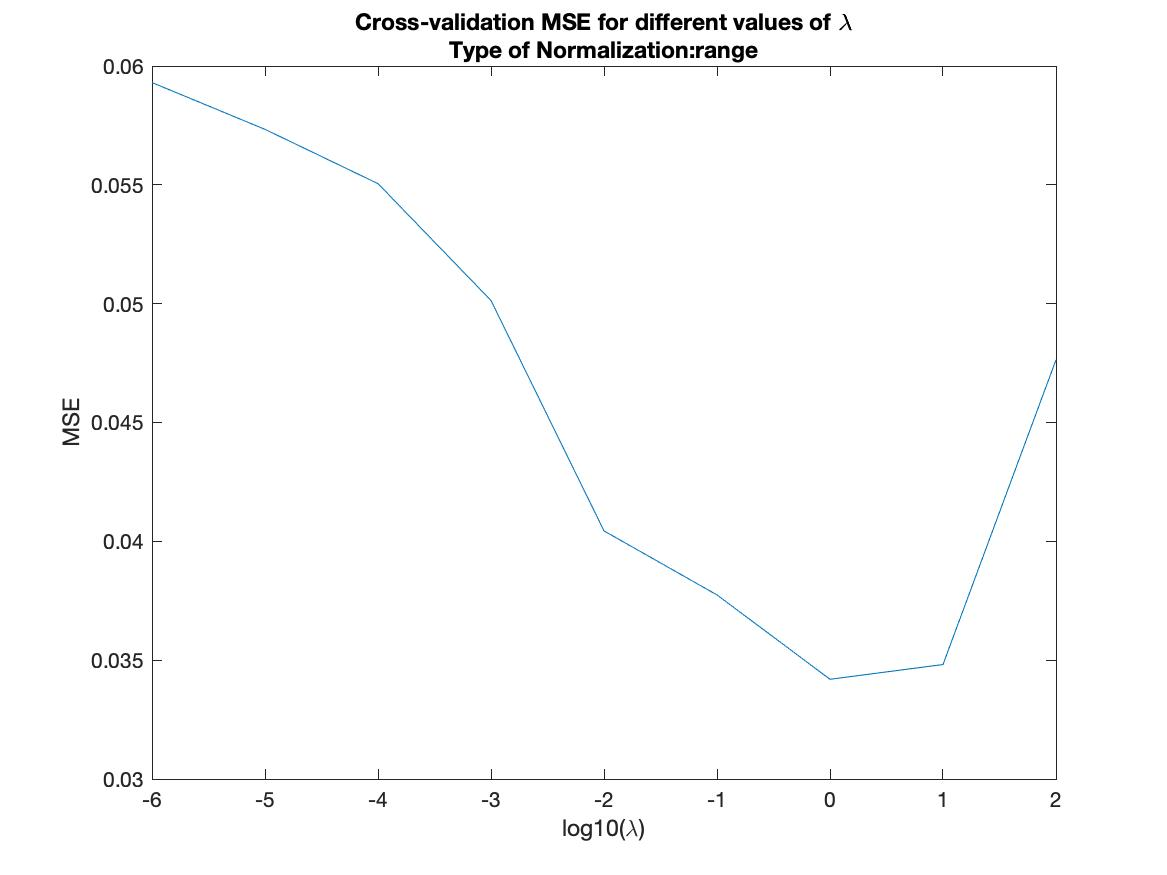
\includegraphics{Codes/MSE_Plots_range.jpg}\\ 
			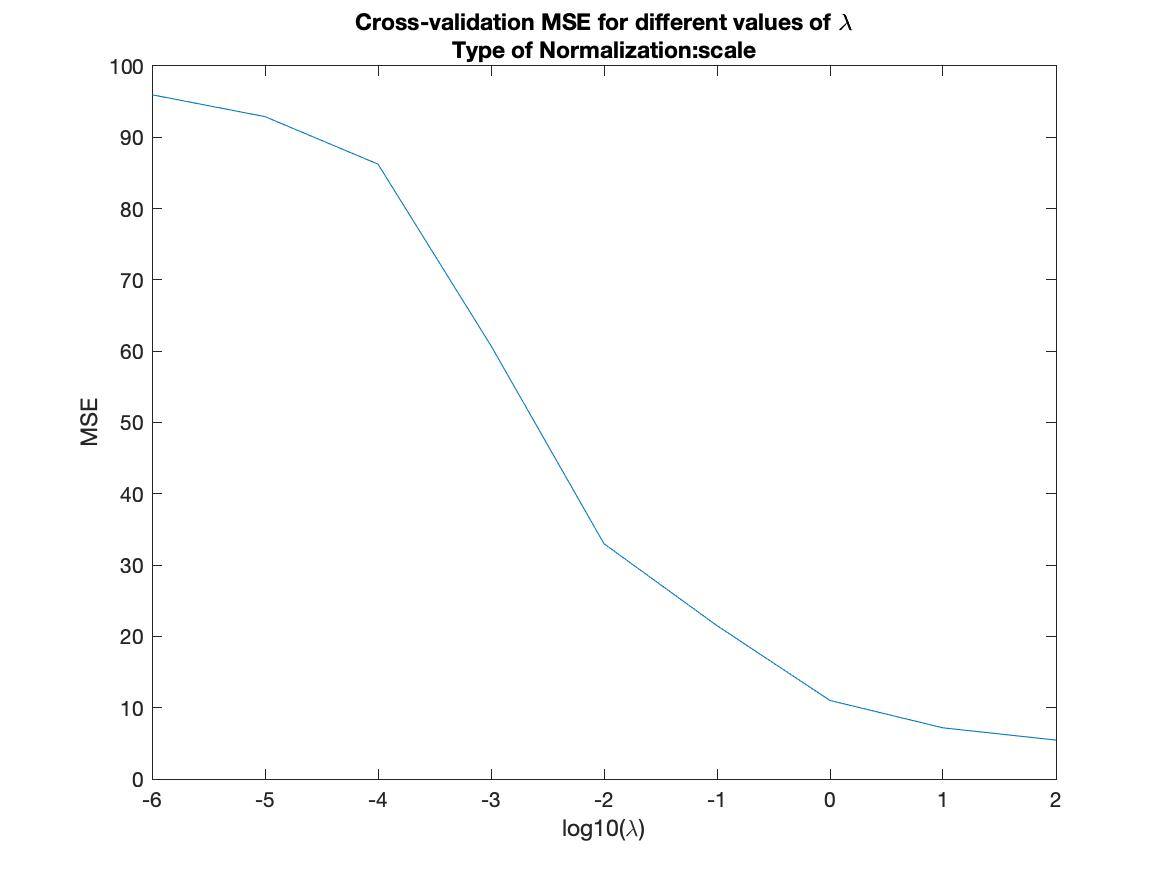
\includegraphics{Codes/MSE_Plots_scale.jpg} & 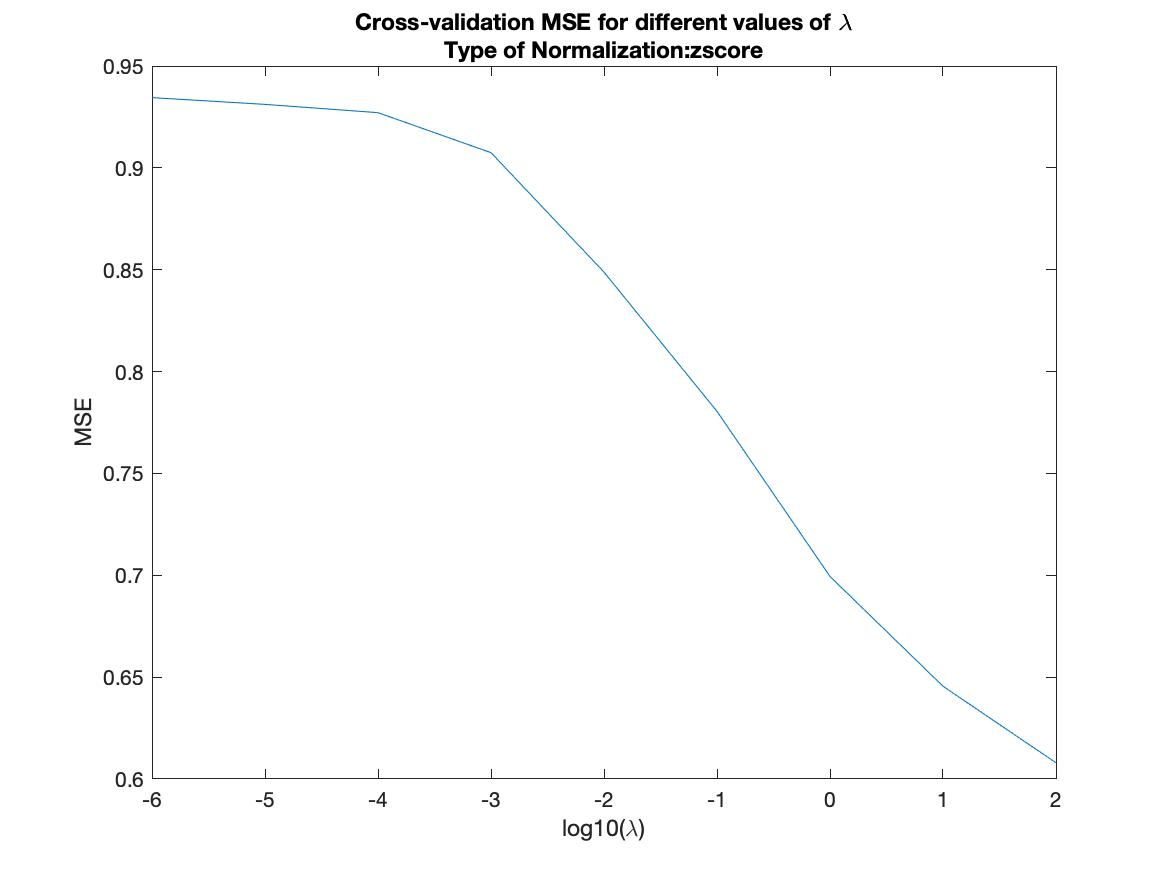
\includegraphics{Codes/MSE_Plots_zscore.jpg}\\
			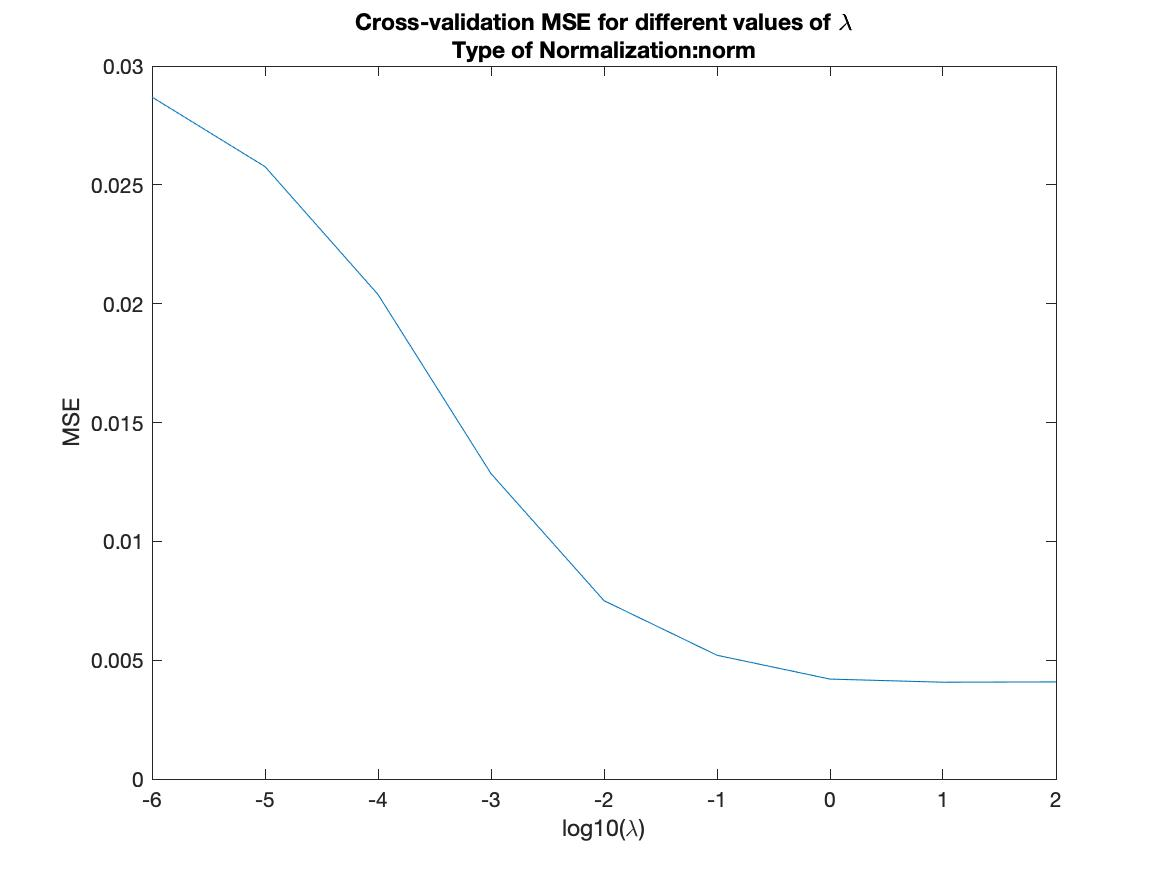
\includegraphics{Codes/MSE_Plots_norm.jpg} & 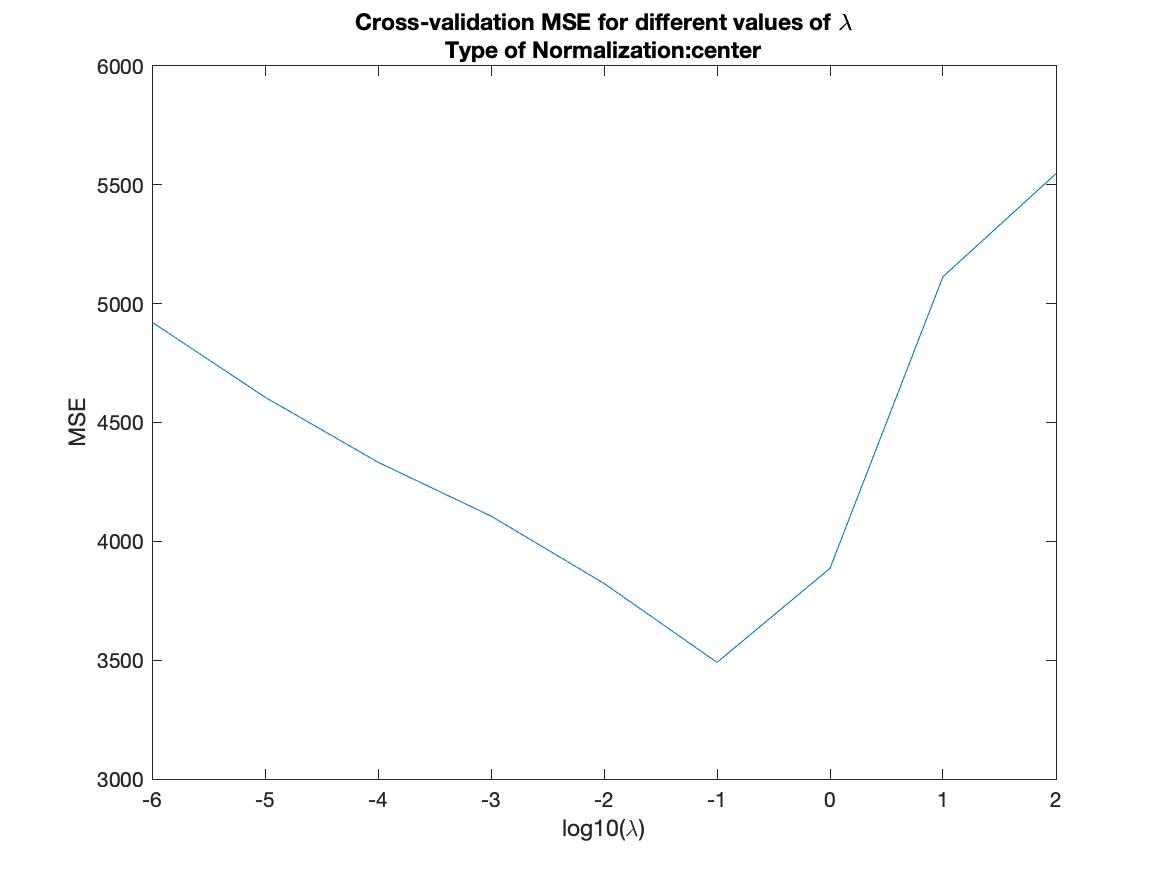
\includegraphics{Codes/MSE_Plots_center.jpg}\\
		\end{tabular}
	\end{adjustbox}
	\caption{Plot of Cross-Validation MSE values for different $\lambda$s for different types of normalizations}
	\label{Fig: MSE_Plot}
\end{figure}

From the Figure, it is visible that different $\lambda$ values are preferred for different normalization techniques. In case of `range' and `center' normalizations, we get a $v$-shaped curve, so it is ensured that we have reached a global optima. In the non-normalized scenario and the `norm' normalization, the MSE stabilizes after $\lambda=10$. For rest of the cases, the MSE value keeps on decreasing even after $\lambda=10$.\\
  
The code used to generate the outcome is provided below. It is also attached to \textit{D2L} as \textbf{RidgeRegSolver.m}.
  
\lstinputlisting[language=Matlab]{Codes/RidgeRegSolver.m}

\end{document}
